\documentclass[11pt,a4paper,titlepage]{article}

\usepackage[utf8]{inputenc}
\usepackage[english]{babel}
\usepackage{csquotes}

\usepackage{listings}
\usepackage{xcolor}
\usepackage[none]{hyphenat}
\usepackage{textcomp}
\usepackage{parskip}

\usepackage{graphicx}
\graphicspath{ {images/} }

%Library
\usepackage[backend=bibtex,style=numeric]{biblatex}
\addbibresource{document.bib}

\setlength{\parskip}{1em}

\begin{document}

%The main goal is that students use this progress report to schedule their work and allow supervisors an opportunity to comment on the approach taken by students and the level of progress made.

	Using an agile methodology will be an important part of the development of this project as it provides a far superior work flow as opposed to far more static methodologies such as the waterfall method. This will result in an improved rate of work and the addition of currently undiscovered ideas.

%Write about requirements

	For a game engine to be a complete engine a wide variety of features are required especially when a high level scripting language is the only input for developers to use when creating a game.

	The engine will provide a Lua interface to all required core engine features using the Lua C API.

	The engine will need the ability to render, reposition, angle and animate sprites provided from a spritesheet.

	Physics will also need to be provided by the engine to allow for much improved performance over having physics implemented in Lua.

	Both the physics and rendering capabilities of the game engine will need to be fully accessed through the provided Lua API. The Lua API should be consistent and easy to use, matching, where possible, the Lua style completely.

%Write about lib choices for each part

	Parts of the engine will be handled by external libraries, an important property of these libraries is performance and modernness as well as cross platform capability. Ideally the libraries will be open source.

	Rendering, physics, scripting and sound will be handled by external libraries and implemented in the game engine. For rendering and sound there are several choices: SDL, SFML, DirectX and OpenGL with a sound library. SDL is widely used and has very good performance but it is written in pure C so has no object oriented code and is therefore quite dated when compared to SFML. DirectX is only available on the windows and Xbox platforms and is therefore not ideal for this project as cross platform is a requirement. OpenGL with a sound library has the best performance of all of the options but is also the most difficult to use and both SDL and SFML wrap OpenGL and provide access to the context so would be better options.

	SFML or Simple and Fast Multimedia Library is written in C++ and is available on Linux, Mac, Windows and FreeBSD and is fully open source with its code available on github. SFML handles everything from window management and input to sound and networking, the performance is very similar to that of SDL but provides a modern object oriented API unlike SDL. These reasons make SFML the perfect choice for the projects requirements.

	For the physics library there is only one real option when it comes to games. Box2d is an open source C++ physics engine for simulating rigid bodies in 2D~\cite{Box2D}. It has excellent performance and is well proven for it's suitability for this project as many games and game engines on all platforms use it to great effect.

	As for scripting the game engine there are several options such as C\#, Javascript and Lua. For the purposes of this project, Lua is the best option due to it's simple binding process and powerful syntax. Many games use Lua as their embedded scripting language such as Garry's Mod, World of Warcraft, Angry Birds and many many more.

%Write what needs to be done and in what order 

	The first step to creating a game engine is to get each of the libraries working correctly in a single project.

	The engine will require a variety of features including an entity management system such as the entity component system, this will allow for dynamic game objects that are easily pieced together by a developer. This system will need to manage a wide variety of entities in various forms including drawing, animating, playing sounds and others. An example entity that will behave as a player controlled car would have the following class diagram, the entity component system example is shown in \ref{fig:ClassDiagram1}.

	\begin{figure}[h] 
		\centering
		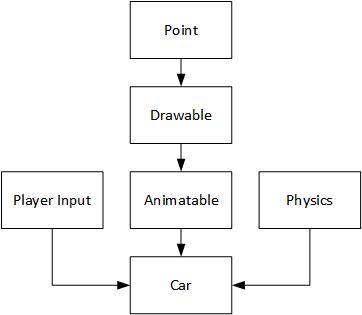
\includegraphics[scale=0.75]{ECS1}
		\caption{ECS Class Diagram Example}
		\label{fig:ClassDiagram1}
	\end{figure}

	For a car to be functional in a game it will need to be drawn and animated, have a physical presence in the world and receive player input. Behaviour can be easily placed into new components when repeated code is required, in the static inheritance system this is not as simple.

	\begin{figure}[h]
		\centering
		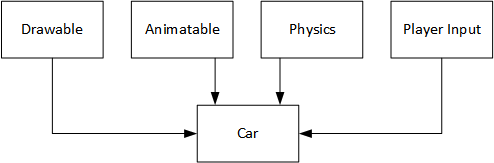
\includegraphics[scale=0.75]{ECS2}
		\caption{ECS Class Diagram Example}
		\label{fig:ClassDiagram2}
	\end{figure}

	Another example of the same in game behaviour in the more traditional class hierarchy system is much simpler to implement but doesn't allow for the dynamism of the entity component system as is shown in \ref{fig:ClassDiagram2} and the diagram is clearly more complicated and may result in repeated code. 

	Lua script management will be entirely handled within the core of the game engine allowing for creating and removing objects, managing object behaviour, physics interactions, UI, the camera and more. The engine will be a completely open source and will be easily expandable and improvable by the community as a result.

	For the UI an external library created to provide UI capabilities to SFML could be used such as SFGUI or TGUI. This will need binding for use in Lua which could prove to be challenging, however getting the minimum working example would not be too difficult. It may be better for the development time if only text rendering is implemented as other UI elements can be achieved using sprites.

	Loading and saving of the game state should be integrated into the game engine to speed up development time for the game developer. Level loading should also be integrated, an external open source level editor application could be used for the creation of the levels, a json or other data file could then be loaded into the game engine reducing the development time even further. Settings should also be managed by the game allowing the Lua developer to load and save any required key value pairs using a provided API, by implementing these features in the game engine the game developer can focus more on the actual game rather than semantics.

	Documentation is a requirement for people to be able to use the engine to create games effectively and helps to reduce the learning curve. Each part of the documentation should be completed after the completion of every Lua accessible feature to ensure that it is kept on top of. Some kind of automatic documentation tool could be used similar to that of Golang's GoDoc or Java's javadoc, this would allow for the the documentation to stay up to date given any changes to the underlying code.

	%Design stuff
	
	Required systems

	SFML Window
	Box2d world
	Resource Manager
	Gamestate Manager
	Lua State

	\printbibliography{}
\end{document}